\chapter{Simulation of a Knowledge Commons with Presage2}

\section{Simulation Setup}

We model a participatory sensing problem as a reinforcement learning problem (See Sutton \& Barto). Policies are knowledge artifacts, which can be appropriated and used to chose actions. Agents are able to measure directly the reward from an action when performing it. Their aim is to maximise rewards over time by training a better policy. All agents play the same game, so policies and measurements are useful for everyone, and one agent's measurements can be used to train another's policy.

As policies will improve with more information, the best strategy for agents will be to pool their information and knowledge together. 
Therefore, by forming an institution around this information and knowledge, everyone should be able to achieve a better utility overall.

%The simulation is set up as a symmetric participatory sensing problem. This is a problem where agents are playing a repeated game where, in each round, a strategy played by the agent yields a reward. Agents are able to measure their previous rewards. They aim to maximise their reward over time by learning the best strategy to choose. As all agents are playing the same game this learning can obviously be improved by gathering together this information. Additionally not all agents will have the knowledge or capability to do this learning themselves. 

The institution is constructed as a provision and appropriation system with two pools. One for information as gathered by the learning agents, and the other for knowledge provided by analysts. This problem is symmetric as each group of agents will provision to one pool and appropriate from the other---learning agents provision information and appropriate knowledge and appropriate information and provide knowledge---thus they are also dependant on each other. If the institution is unsatisfactory for one group and they leave it will quickly become unsatisfactory for the others too.

The utility generated from the learning problem acts as the only external input of value into the system, while paying for facility costs is the only way of value flowing out of the system. All other transactions are endogenous. There is also a possibility, as seen in many real-world participatory sensing systems, of other exogenous rewards from ownership of a data-set, however we do not simulate this.

\subsection{Rewarding Knowledge}

In order to model the additive value of information when combined for learning we use an artificial reward function which gives a utility proportional to the quality of policy used to chose an action. The quality of a policy is defined as the number of information samples over a time window from the current time:

A policy is a tuple containing a set of data samples: $P = <S>$. A predictor can recommend an action for an agent: $\mathit{selectAction}(P,t) \rightarrow s_t$. Using this action then yields a reward: $u(s_t) = \sum_t^{t-W} \frac{|S_t|}{W*N}$ where $W$ is a time-window size for which information is useful and $N$ is maximum number of samples possible in one time-step. This function returns a value between 0 and 1.

\subsection{Agent strategies}

\begin{itemize}
\item Sustainable
\item Profitable
\item Greedy
\end{itemize}

\section{Experiments}

\subsection{The Problem of Supply}\label{sec:supply}

This first set of experiments looks at the problem of provisioning an institution for the problem we have outlined. Despite having a simple game where we can seemingly trivially generate utility, getting together disparate agents to all contribute and keeping it sustainable over the long time requires negotiating several hurdles. 

We will see these hurdles as we follow the process of building a centralised institution for this problem. This institution has a single agent who acts as a manager for the institution and as complete control over institutional fluents.

The experimental setup is as follows:
\begin{itemize}
\item One institution with information and knowledge pools.
\item 10 gatherer/consumer agents who are members of the institution.
\item One analyst agent providing knowledge for the institution.
\item One initiator agent managing the institution.
\item One independent agent as a control benchmark. This agent has the same knowledge as the analyst, but only uses self-gathered information.
\end{itemize}

\subsubsection{Facility Cost}

Storing information and knowledge, and other infrastructure required for the institution will incur facility costs. We have two profiles to model facility costs:
\begin{itemize}
\item High sunk cost --- A high initial sunk cost (for infrastructure acquisition), followed by a lower fixed cost each time-step ($\mathtt{sunk\_cost}=50$, $\mathtt{fixed\_cost}=1$).
\item High fixed cost --- No initial sunk cost, higher fixed cost ($\mathtt{sunk\_cost}=0$, $\mathtt{fixed\_cost}=2$).
\end{itemize}

We are running simulations over 200 time-steps, so these profiles would correspond to a total incurred cost of 250 and 400 respectively.

\begin{figure}
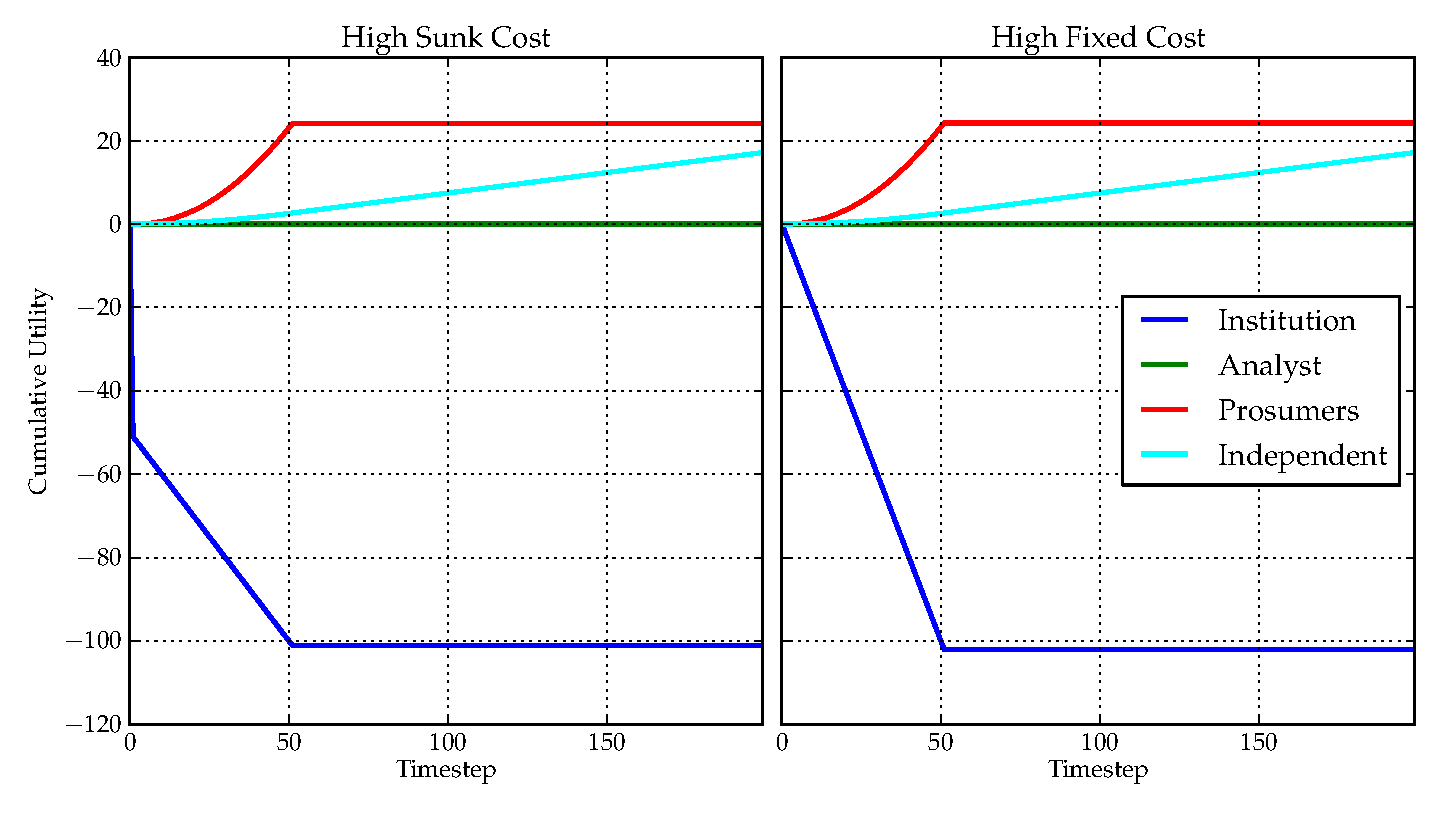
\includegraphics[width=\linewidth]{gfx/kc/facility1v2.pdf} 
\caption{Cumulative agent utilities over time in basic centralised institution with high--sunk and high--fixed facility profiles.}\label{fig:facility1}
\end{figure}

Figure~\ref{fig:facility1} shows the utilities in this scenario. In both cases the institution runs out of resources to pay for facilities after 50 timesteps, at which point the institution ceases to function. As the in-flow of utility into the system (to prosumers) is separate from where the facility is paid for (by the initiator) then the system cannot endure without the charity of the initiator. Therefore without exogenous income for this agent we require a way for prosumers to contribute to the facility costs.

One method we can use is to have a subscription fee. This is a payment to the institution each timestep which one is occupying a certain role. The level of this fee is determined by the initiator who has the sole power to set its value. 

\begin{figure}
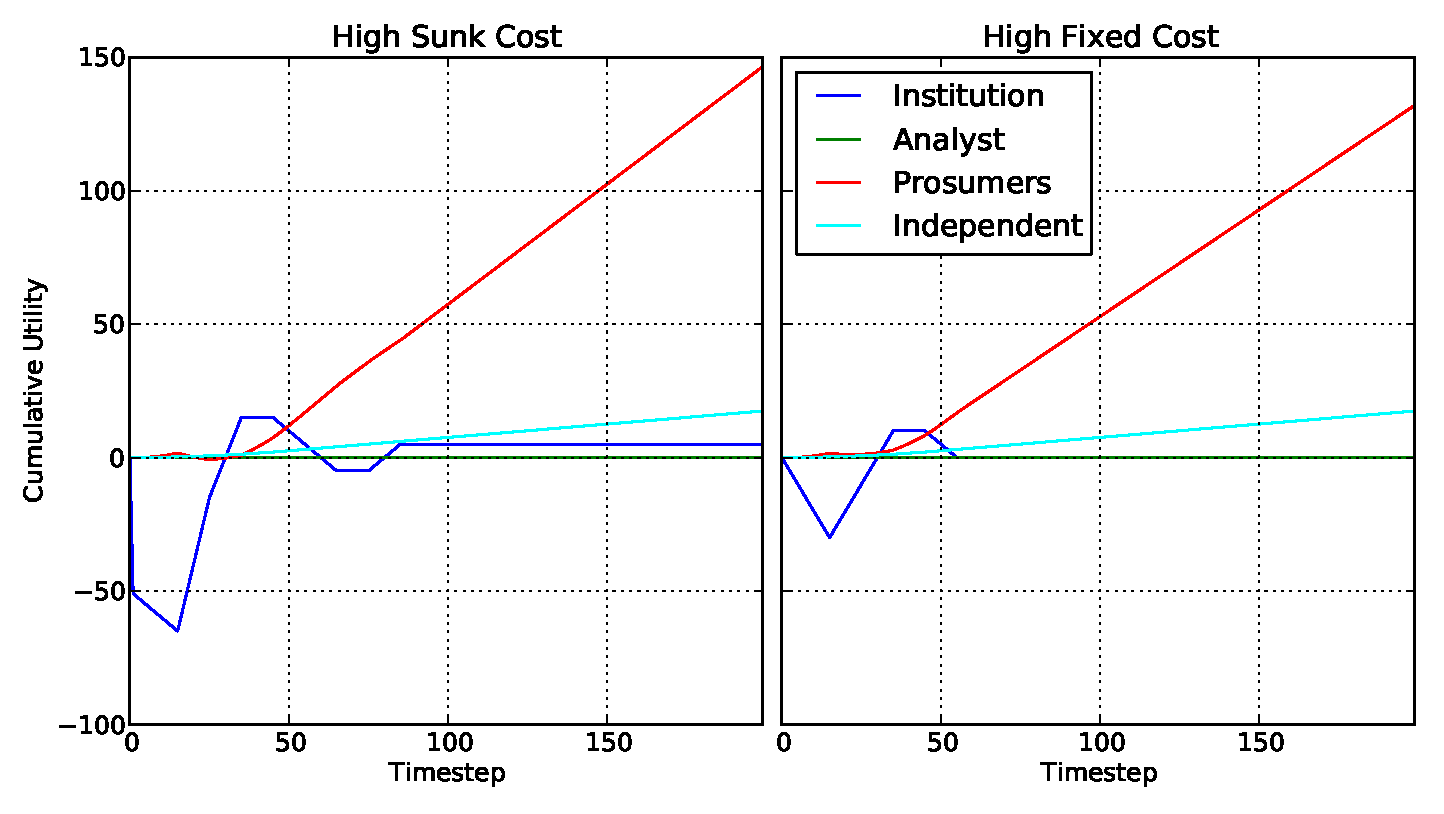
\includegraphics[width=\linewidth]{gfx/kc/facility2.pdf} 
\caption{Cumulative agent utilities over time in centralised institution using subscription fees with high--sunk and high--fixed facility profiles.}\label{fig:facility2}
\end{figure}

Figure~\ref{fig:facility2} shows agent utilities once subscription fees are introduced. The rate dynamically adjusts to ensure that the institution breaks even and that the institution endures. Here we also see the benefit of the institution. Prosumer agents accrue over 7.5 times more than the independent control agent in each case due to having 10 times more data and only small additional overheads.

\subsubsection{Compensating Analysts}

Figures~\ref{fig:facility1}~\&~\ref{fig:facility2} from the previous section both show zero utility gained for the analyst agent. However are having to appropriate information and process it in order to generate the knowledge which they provision. Given that this knowledge enables a large increase in reward for the prosumer agents, analysts may expect some remuneration.

This can be achieved by paying an analyst when knowledge is appropriated. Again the initiator can set the rate for this payment. Table~\ref{tab:analyst1} shows final utilities for agents when a fixed rate of 0.1 per appropriation is set.

\begin{table}
\centering
\begin{tabular}{c|c||c|c}
Facility Profile & Pay Analysts? & Prosumers & Analyst \\ 
\hline \hline
High sunk & no & 142 & 0 \\ 
\hline 
High sunk & yes & 127 & 157 \\ 
\hline 
High fixed & no & 128 & 0 \\ 
\hline 
High fixed & yes & 112 & 144 \\ 
\end{tabular}
\caption{Compensation of analysts}\label{tab:analyst1}
\end{table} 

\subsubsection{Compensating Gatherers}

In the previous examples all prosumers always gather information, and always provision it, as there is no cost for them in this process. However in some cases there is likely to be some costs associated with gathering information. In turn this may cause some agents to `free-ride' by not gathering or provisioning information while still receiving the benefits of the institution. Again we can simply introduce a payment for provision or appropriation of this information.

\begin{table}
\centering
\begin{tabular}{c|c|c||c|c|c}
Facility Profile & Pay Gatherers? & No. Greedy & Compliant & Non-compliant & Analyst \\ 
\hline \hline
High sunk & no & 2 & 74 & 93 & 157 \\ 
\hline 
High sunk & no & 5 & -8 & -1 & -8 \\ 
\hline
High sunk & yes & 2 & 91 & 92 & -4 \\ 
\hline 
High sunk & yes & 5 & 92 & 91 & -4 \\ 
\hline  
High fixed & no & 2 & 61 & 81 & 144 \\ 
\hline 
High fixed & no & 5 & -8 & -10 & -2.5 \\ 
\hline
High fixed & yes & 2 & 67 & 64 & -4 \\ 
\hline 
High fixed & yes & 5 & 64 & 68 & -4 \\ 
\end{tabular}
\caption{Compensation of gatherers with measuring cost of 0.1}\label{tab:gatherers1}
\end{table} 

Table~\ref{tab:gatherers1} shows cumulative utility for compliant and non-compliant prosumers, and analysts when a measuring cost is introduced. Non-compliant prosumers will not generate information to provision if it is not profitable to do so (payment for provision less than measuring cost). The data shows that introducing a payment to gatherers reduces this non-compliant behaviour. However the knock-on effect is that it is more expensive for the analyst to operate, and in fact this agent cannot afford to appropriate all of the available information as before. This results in lower quality knowledge and less total utility generated by the system.

This problem can be prevented by simply increasing the pay to the analyst for appropriations. Figure~\ref{fig:measuringCost} shows the average cumulative utilities for each agent group with three institution configurations:
\begin{enumerate}
\item Without payment to gatherers.
\item With payment to gatherers.
\item With payment to gatherers and increased payment to analyst.
\end{enumerate}
Each configuration is tested with two and five non-compliant prosumers out of the ten total.

\begin{figure}
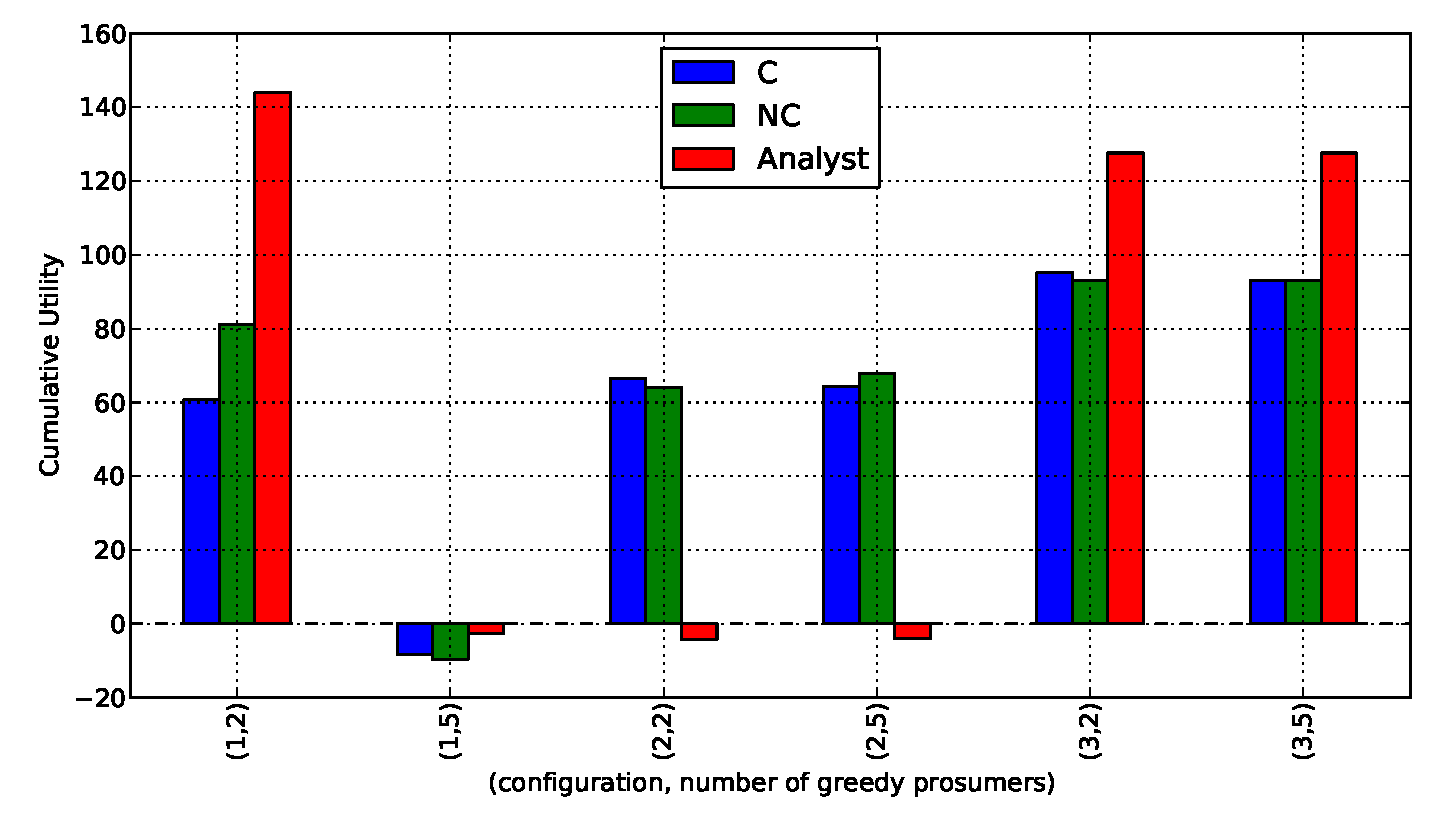
\includegraphics[width=\linewidth]{gfx/kc/measuringCost1.pdf} 
\caption{Average cumulative utilities for Compliant prosumer (C), Non-compliant prosumer (N) and Analyst groups under three institution configurations and with 2 and 5 N agents.}\label{fig:measuringCost}
\end{figure}

From the graph we can see that properly compensating the analyst allows for better knowledge to be generated.

\subsection{Self-Organisation}

We have seen in the previous section that we require several mechanisms in place to create an effective institution. Using static examples allows us to test certain situations, however for long-term robustness we require that these fluents, such as subscription fees, and provision and appropriate fees, can be changed over time to react to external and internal conditions. We also require that the agents in the system can do this themselves, without external supervision, so that the system is self-organised.

We do this by allowing these fluents to be changed by vote. Periodically agents are permitted to vote on the value of a fluent, and if the vote is decisive, the value is changed. With this method we can define three models of institutional governance:
\begin{itemize}
\item Centralised --- A single agent has the power to vote on all issues.
\item Market --- Those who provision an artifact (i.e. supply) have the power to vote on its price.
\item Principled --- Following Ostrom's third principle, those affected by an operational rule are permitted to vote on it: Anyone with provision or appropriation rights to a pool can vote on its fees.
\end{itemize}

\subsection{Centralised}

With centralised governance the initiator agent has control over subscription, gatherer pay, and analyst pay rates. Figure~\ref{fig:centralised1} shows a combination of:
\begin{itemize}
\item Setting subscription rates to cover facility costs.
\item Setting a fair appropriation fee to compensate analysts.
\item Setting a reward for provisions when there is a measuring costs to incentivise provisions.
\end{itemize}

\begin{figure}
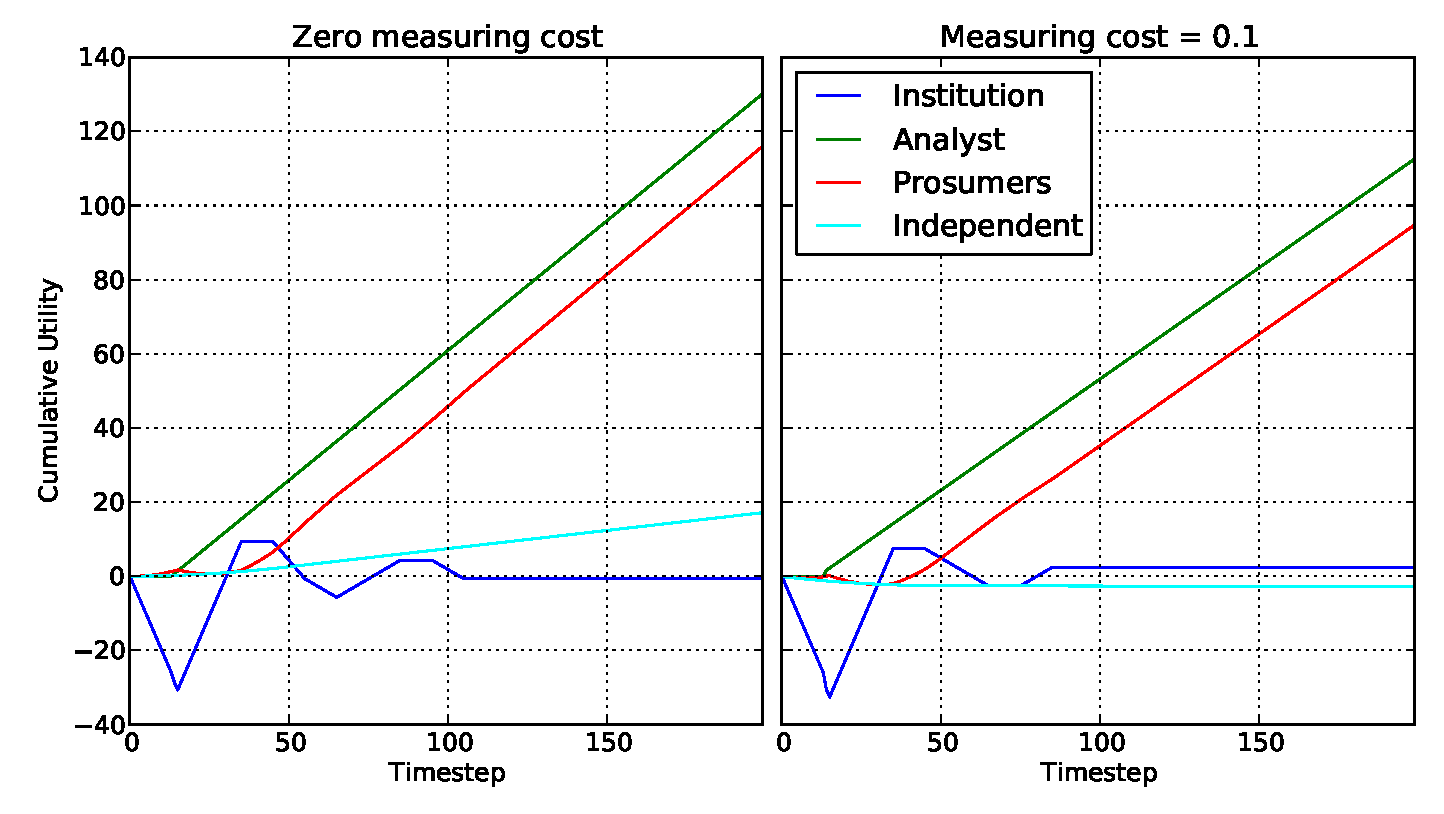
\includegraphics[width=\linewidth]{gfx/kc/centralised1.pdf} 
\caption{Cumulative utility of agent groups over time with centralised governance, and zero and 0.1 measuring cost. Facility profile is high fixed.}\label{fig:centralised1}
\end{figure}

\subsubsection{Market}

To model a basic market scenario we allow artifact suppliers to vote on the appropriation fee for their wares. Facility costs are shared by all agents.

Figure~\ref{fig:market1} shows that the market is less efficient and robust than centralised governance. This is largely due to difficulties in the early stages of the simulation. Both analysts and prosumers are struggling to make a profit, and so raise their prices. This, in turn, means that analysts cannot afford to appropriate all available information, leading to worse knowledge for the prosumers. This effect is even more pronounced when the introduction of measuring costs further increase the scarcity of utility at the start of the simulation.

\begin{figure}
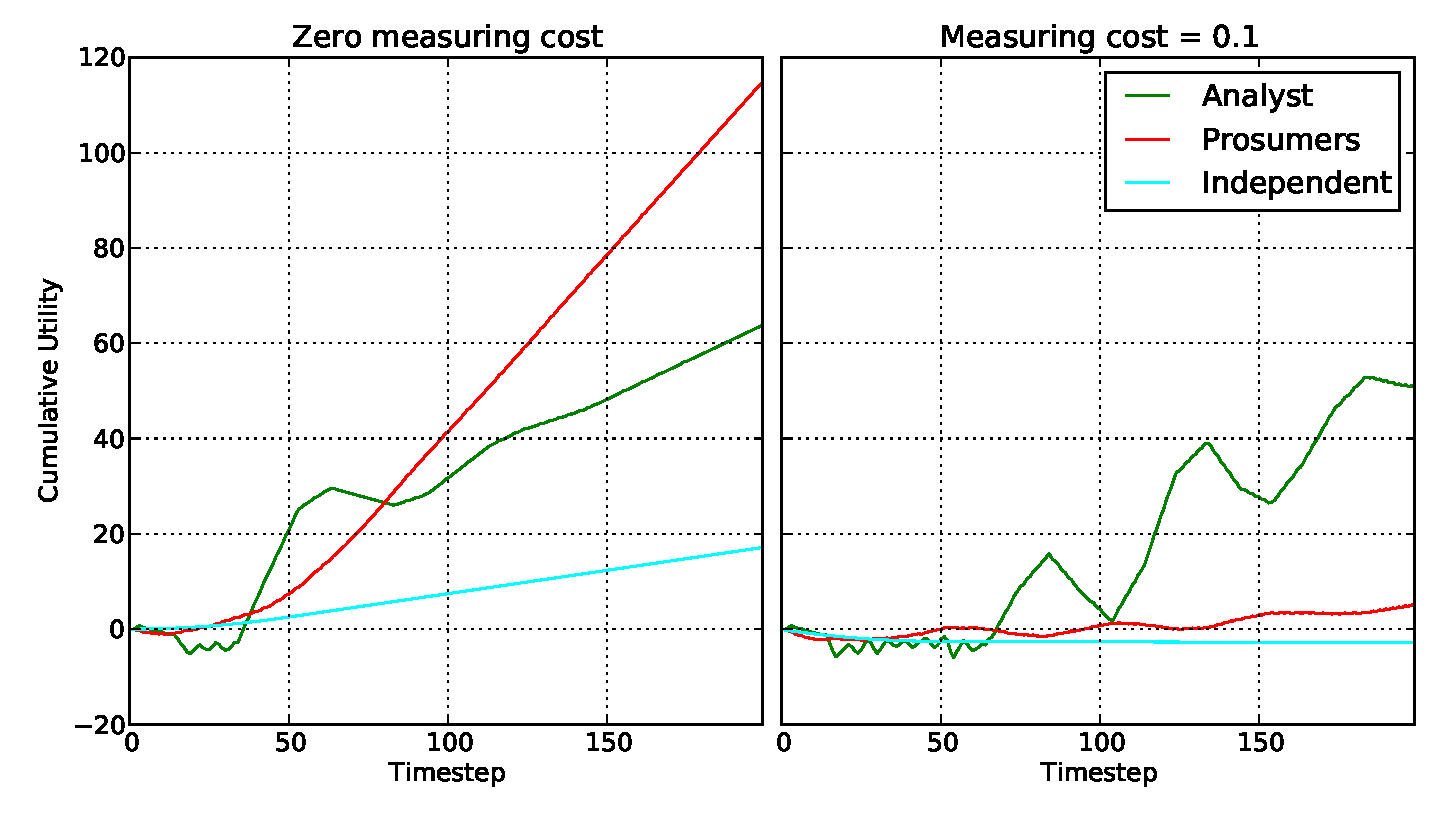
\includegraphics[width=\linewidth]{gfx/kc/market1.pdf} 
\caption{Cumulative utility of agent groups over time with a market, and zero and 0.1 measuring cost. Facility profile is high fixed.}\label{fig:market1}
\end{figure}

\subsubsection{Principled}

Under this governance scheme both analysts and prosumers can vote on appropriation rates for artifacts and a subscription fee for the institution. In order to prevent these votes being biased towards group, the ballot is weighted such that each group has an equal weighting across all its voters. Thus the vote represents a compromise across the preferences of the two groups.

Figure~\ref{fig:principled1} shows that this governance functions comparably to centralised in compensating agents.

\begin{figure}
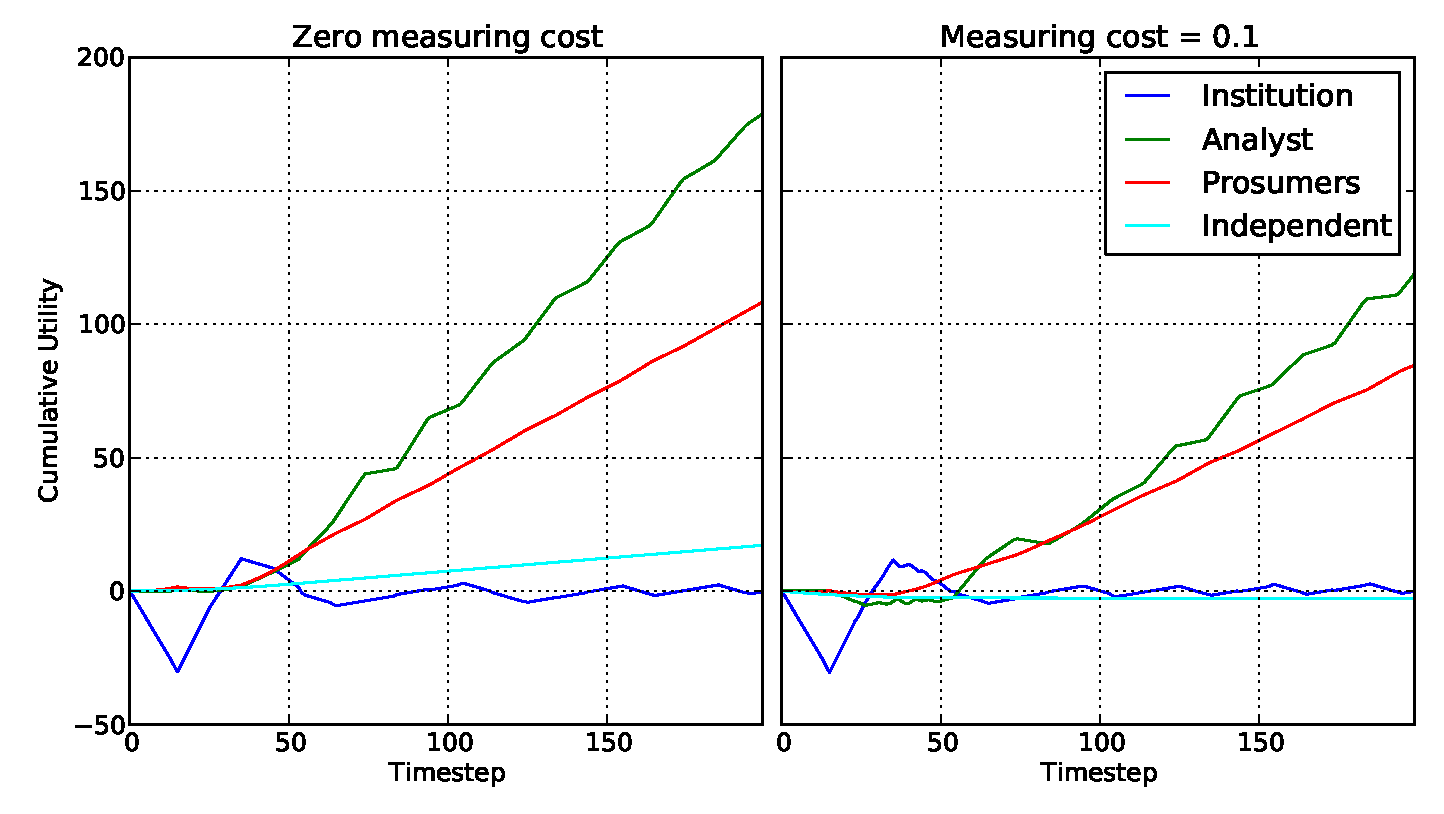
\includegraphics[width=\linewidth]{gfx/kc/principled.pdf} 
\caption{Cumulative utility of agent groups over time with collective governance according to Ostrom's third principle, and zero and 0.1 measuring cost. Facility profile is high fixed.}\label{fig:principled1}
\end{figure}

\subsection{Comparison of institutional paradigms}

We will not compare the three institutional paradigms with respect to the effect that malicious agent strategies can have on the institution.

\subsubsection{Individual Power}

How much difference can one agent changing strategy make? Figure~\ref{fig:powerbar} shows the difference in final utilities when individual agent strategies are changed to greedy ones. 

In a centralised regime only the initiator agent can affect the outcome, and he is able to extract significant utility for himself from the other participants. In the market-based case analysts are able to improve their score with more aggressive pricing, but prosumers are unable to benefit themselves - largely as too aggressive pricing causes the knowledge they appropriate to be worse. Finally, with principled governance no individual is able to benefit themselves, however a selfish majority of prosumers can significantly impact the analyst's utility.

\begin{figure}
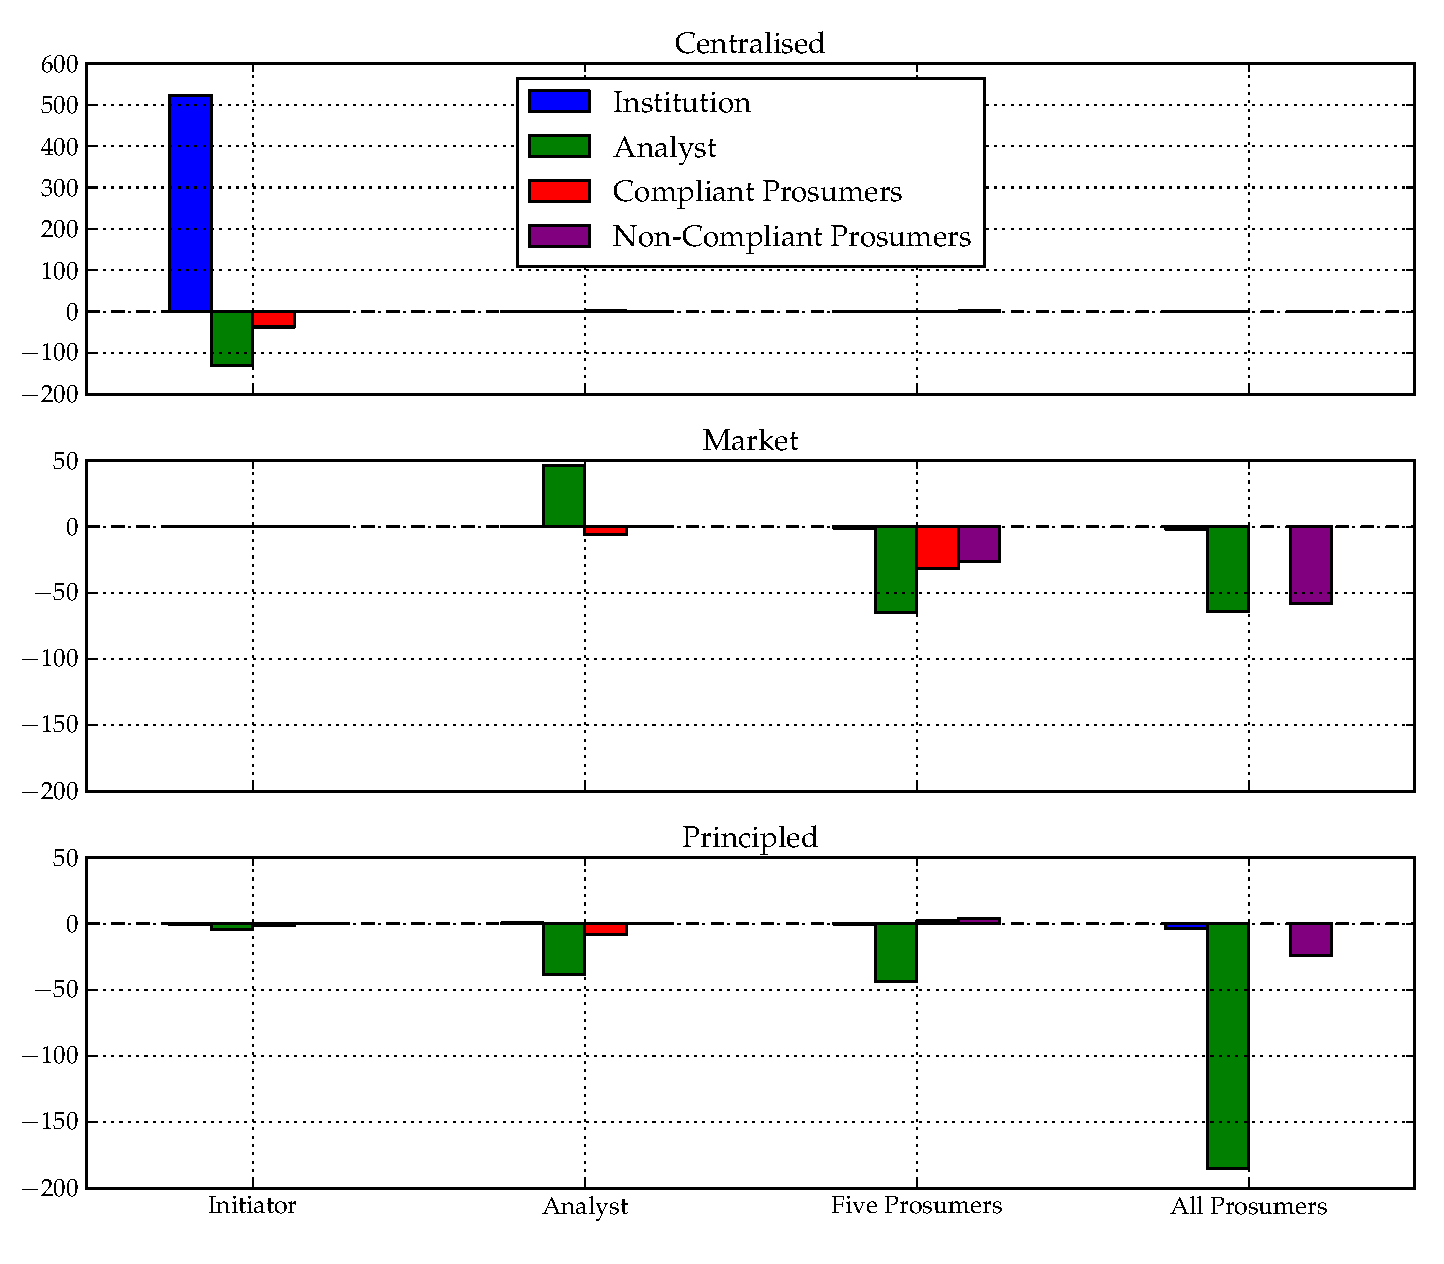
\includegraphics[width=\linewidth]{gfx/kc/powerbarv2.pdf} 
\caption{Change in final utilities of agent groups when individuals change to a greedy strategy.}\label{fig:powerbar}
\end{figure}

From this we can conclude that both market and principled paradigms are much better at preventing self-interested individuals from exploiting the system, and also dis-incentivising non-cooperative behaviours.

\section{Evaluation \& Conclusions}

\begin{itemize}
\item The problem of supply: Institutions are hard to set-up, particularly early on.
\item Compensating desired roles: require self-organising mechanisms to incentivise desired behaviours.
\item Concentration of power: Too much power given to an individual can allow them to unfairly influence others' outcomes.
\item Centralised allows the \emph{initiator} agent to extract profit at will.
\item Market: price competition generally cancels out and also mostly prevents concentrated power. NC agents kept interested by compensation for provisions.
\item Collective: Robust to malicious agent strategies. Requires appropriate voting rules (weighted in this case).
\end{itemize}